% 2020 全国Ⅱ卷 文3：钢琴键盘局部示意图（12 个键 a1—a12）
% 来源 PDF：普通高考/2020/2020全国2文(…).pdf 第 1 页（A3 横排），印面 1123，第 3 题题干下方
% 结构：七个白键 a1、a3、a5、a6、a8、a10、a12 自左至右排列；
%       五个黑键 a2、a4、a7、a9、a11 分别骑在相邻两白键的分界处，短于白键并从顶端下垂；
%       a5 与 a6 之间（第 3、4 个白键之间）没有黑键，对应键盘上 E—F 的半音间隙。
% 尺寸比：黑键宽 = 白键宽 × 2/3，黑键高 = 白键高 × 0.563（按原页 300 dpi 量取）。
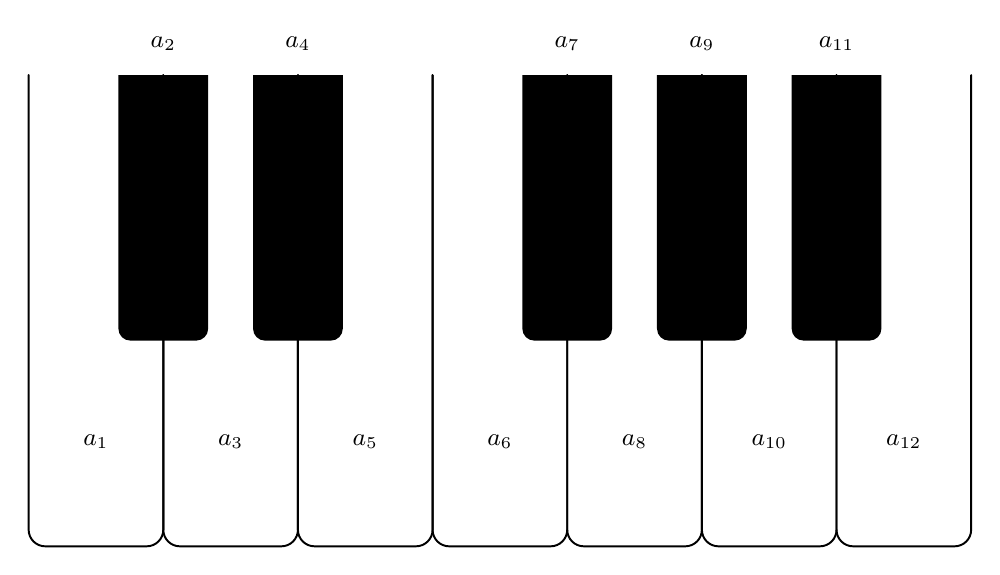
\begin{tikzpicture}[line width=0.7pt, font=\small,
  x=0.95cm, y=0.95cm, line cap=round, line join=round]
  \def\kw{1.8}    % 白键宽
  \def\kh{6.3}    % 白键高
  \def\bw{1.2}    % 黑键宽
  \def\bh{3.55}   % 黑键高

  % 白键：只画两侧竖线与圆角下沿，顶端不封口
  \foreach \i/\lab in {0/a_1, 1/a_3, 2/a_5, 3/a_6, 4/a_8, 5/a_{10}, 6/a_{12}} {
    \draw[rounded corners=6pt]
      ({\i*\kw},0) -- ({\i*\kw},-\kh) -- ({\i*\kw+\kw},-\kh) -- ({\i*\kw+\kw},0);
    \node at ({\i*\kw+\kw/2},-4.9) {$\lab$};
  }

  % 黑键：骑在白键分界处，实心，顶端齐平、下沿圆角
  \def\br{0.16}   % 黑键下沿圆角半径
  \foreach \b/\lab in {1.8/a_2, 3.6/a_4, 7.2/a_7, 9.0/a_9, 10.8/a_{11}} {
    \fill ({\b-\bw/2},0)
      -- ({\b-\bw/2},{-\bh+\br})
      arc[start angle=180, end angle=270, radius=\br]
      -- ({\b+\bw/2-\br},{-\bh})
      arc[start angle=270, end angle=360, radius=\br]
      -- ({\b+\bw/2},0) -- cycle;
    \node at ({\b},0.42) {$\lab$};
  }
\end{tikzpicture}
